\documentclass[12pt]{article}

\date{Mai 2018}
\usepackage[francais]{babel}
\frenchbsetup{StandardLists=true}
\usepackage{extsizes}
\setlength{\parskip}{\baselineskip}
\usepackage{natbib}
\usepackage{geometry}
\geometry{hmargin=2cm,vmargin=2.5cm}
\usepackage[utf8x]{inputenc}
\usepackage{amsmath}
\usepackage{graphicx}
\usepackage[colorinlistoftodos]{todonotes}
\usepackage{enumitem} 
\usepackage{booktabs}% http://ctan.org/pkg/booktabs
\newcommand{\tabitem}{~~\llap{\textbullet}~~}
\usepackage{hyperref}
\usepackage[utf8]{inputenc}
\usepackage{minted}
\usepackage[frenchb]{babel}
\usepackage[utf8]{inputenc}
\usepackage[T1]{fontenc}
\usepackage{charter}
\usepackage{graphicx}
\usepackage{amsmath}
\usepackage{amsfonts}
\usepackage{stmaryrd}
\usepackage{diagbox}
\usepackage{amsthm}
\usepackage{textcomp}
\usepackage[a4paper,margin=1in]{geometry}

\usepackage{comment}

\begin{document}

\begin{titlepage}

\newcommand{\HRule}{\rule{\linewidth}{0.5mm}} % Defines a new command for the horizontal lines, change thickness here

\center % Center everything on the page
 
%----------------------------------------------------------------------------------------
%	HEADING SECTIONS
%----------------------------------------------------------------------------------------

\textsc{\LARGE École Nationale des Ponts et Chaussées}\\[1.5cm] % Name of your university/college
\textsc{\Large Projet de Département IMI}\\[0.5cm] % Major heading such as course name

%----------------------------------------------------------------------------------------
%	TITLE SECTION
%----------------------------------------------------------------------------------------

\HRule \\[0.4cm]
{ \huge \bfseries Gen Slides}\\[0.4cm] % Title of your document
\HRule \\[1.5cm]
 
%----------------------------------------------------------------------------------------
%	AUTHOR SECTION
%----------------------------------------------------------------------------------------

\begin{minipage}{0.4\textwidth}
\begin{flushleft} \large
\emph{Partners:}\\
Louis \textsc{Montaut}\\ Matthieu \textsc{Moreau}\\ Hugo \textsc{Senetaire}
\end{flushleft}
\end{minipage}
~
\begin{minipage}{0.4\textwidth}
\begin{flushright} \large
\emph{Senior Advisor:} \\
Benoit \textsc{FRANCK} % Supervisor's Name
\end{flushright}
\end{minipage}\\[2cm]
%----------------------------------------------------------------------------------------
%	DATE SECTION
%----------------------------------------------------------------------------------------

{\large \today}\\[2cm] % Date, change the \today to a set date if you want to be precise

%----------------------------------------------------------------------------------------
%	LOGO SECTION
%----------------------------------------------------------------------------------------

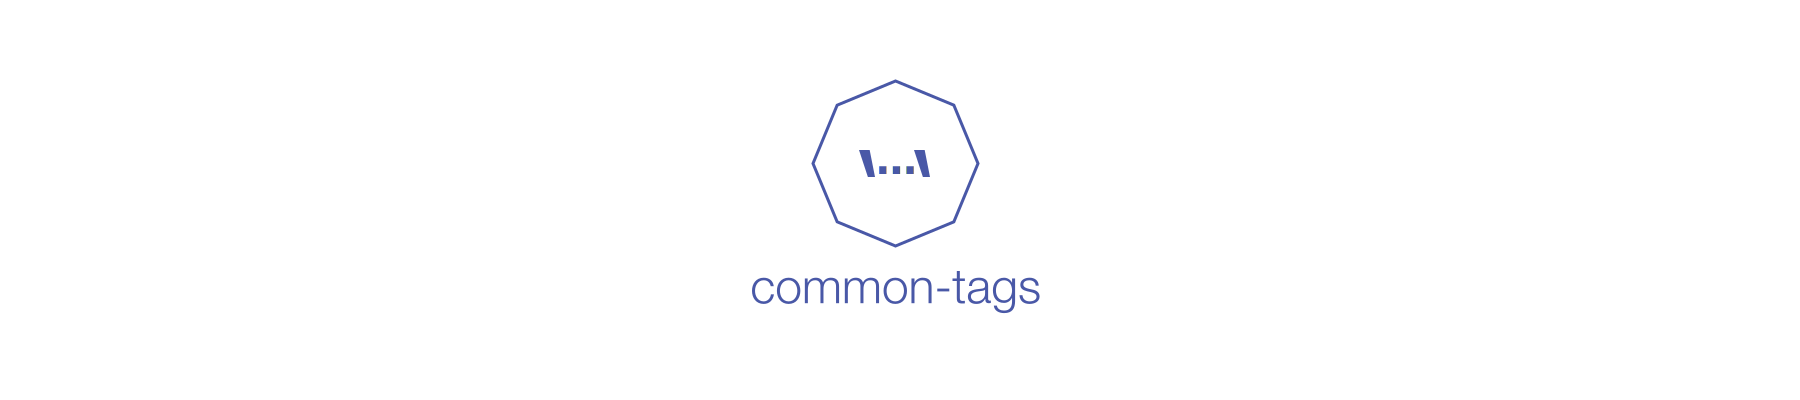
\includegraphics{logo.jpg}\\[1cm] % Include a department/university logo - this will require the graphicx package
 
%----------------------------------------------------------------------------------------

\vfill % Fill the rest of the page with whitespace

\end{titlepage}

\section*{Remerciements}
Nous remercions nos tuteurs Monsieur Benoit Franck, Monsieur Mohammed El Rhabi pour leur aide, leurs conseils, l’intérêt qu’ils ont montré pour notre projet, et la bienveillance avec laquelle ils nous ont guidés. Nous remercions également l'ensemble des étudiants, chercheurs et/ou enseignants qui ont pris le temps de répondre à notre questionnaire ou qui nous ont fournis des conseils pour améliorer notre projet.
\newpage


\tableofcontents

\newpage

\section{Héritage du patrimoine de l'ancienne équipe}

Le projet "Générateur de Slides" était un projet initialement proposé aux étudiants de première année de l'école des Ponts en 2017. Six étudiants de première année avaient alors travaillé au développement de \textit{Mynima}. A la vue du succès de ce projet, le département IMI a proposé en 2018 le même sujet à ses élèves de deuxième année. Ce projet mêlant des domaines très variés, du développement logiciel jusqu'à l'analyse de texte, nous avons décidé de nous plonger à notre tour dans son développement.

\subsection{Héritage}
La première étape du projet de cette année a donc été l'étude du projet de l'année dernière : lecture du rapport, de l'étude marché, compréhension du code et  application. 

L'application héritée était un générateur automatique de slides qui prenait en entrée un document Word suivant la sémantique Word. L'application analysait ce document et remplissait un document XML structuré à partir duquel une présentation PowerPoint était générée et envoyée à l'utilisateur.

L'application utilisait le modèle SaaS (Software as a Service) en mettant à disposition des utilisateurs un site internet sur lequel ils pouvaient mettre en ligne leur document Word. Le site leur proposait alors de télécharger la présentation automatiquement générée.

\begin{center}
    \centering
    \includegraphics[width=10cm]{screenMynima.png}\\
    Application Mynima
\end{center}

\subsection{Impasse}

Après nettoyage du code, nous avons réfléchi aux pistes d'améliorations potentielles de ce logiciel en nous inspirant des propositions d'amélioration du rapport de l'année précédente. Elles comprenaient les idées principales suivantes : 

\begin{itemize}
    \item Texte en entrée qui n'utilise pas la sémantique Word (détection automatique de titres et des paragraphes)
    \item Analyse des paragraphes au niveau local (pour comprendre le sens du paragraphe) et au niveau global (pour inscrire le paragraphe dans le contexte de la présentation)
    \item Détection et analyse des connecteurs logiques
    \item Détection de chiffres et création automatique de graphiques adaptés
\end{itemize}

Nous avions également envisagé de toutes nouvelles fonctionnalités pour généraliser l'utilisation de l'outil : synthèse de plusieurs présentations en une seule, suggestions de mise en page/templates adaptés, suggestions de présentations sur le même thème trouvées sur Internet.

L'ensemble de ses fonctionnalités s'inscrivaient dans l'optique d'un outil complètement automatique sans intervention de l'utilisateur (outre en entrée et en sortie) telle qu'elle avait été définie dans le projet initial. 

Nous avons alors cherché à développer ces fonctionnalités en élaborant un planning et différentes versions objectifs. Cependant, le développement s'est révélé ardu et plus lent que prévu : les fonctionnalités que l'on cherchait à développer étaient de très haut niveau et demandaient parfois une compréhension automatique du langage naturel qui dépassait l'état de l'art. Nous nous sommes alors rendu compte que le développement d'un outil à la fois automatique et robuste était hors de notre portée et que les présentations générées par notre outil dans sa forme actuelle étaient et resteraient peu satisfaisantes.

\section{Nouveaux clients, nouveaux besoins}

\subsection{Rencontre avec des chercheurs du CERMICS}
C'est à ce moment là que nous avons rencontré les chercheurs du Cermics à qui nous avons présenté notre projet. Ils nous ont également fait part de leur doute quant à l'avenir du projet sous sa forme actuelle. Ils nous ont alors présenté leur propre perspective et leurs besoins en tant que chercheurs et enseignants habitués à présenter des documents pour des conférences ou des cours. Ils nous ont expliqué leur scénario typique : ils commencent par un document LaTeX puis créent une présentation à partir de ce document. Ils doivent alors parcourir l'entièreté du document rédigé, trouver les parties pertinentes, les copier-coller dans un Beamer (code de LaTeX pour des Slides). Tout ceci constitue une perte de temps importante pour des personnes tant qualifiées.

\subsection{Nouveaux besoins}

A partir de ces nouvelles idées, nous avons construit un questionnaire que nous avons envoyé aux différents chercheurs de l'école. Les réponses au questionnaire nous ont permis de définir l'ensemble des besoins et des fonctionnalités pour y répondre. On doit partir d'un document LaTeX  et utiliser notre outils comme aide pour produire une présentation sous forme de Slides.
Les besoins que nous avons détectés sont :
\begin{itemize}
    \item Personnalisation - L'utilisateur doit pouvoir exercer un contrôle total sur la présentation finale
    \item Intuitivité - L'utilisateur doit être capable de comprendre le fonctionnement de l'application en un clin d'oeil
    \item Gain de Temps - L'utilisation du logiciel doit être significativement plus rapide que la création d'un Beamer de toute pièce
    \item Utilisation de LaTeX - Langage de programmation connu et maîtrisé par une grande majorité de chercheurs
    \item Universalité - L'outil doit être accessible facilement et sur toutes les machines 
\end{itemize}
On a donc décidé de réaliser une Web-Application (universalité) qui sert d'assistance à la création de Slides (personnalisation) en facilitant l'accès aux données importantes du document source (Gain de temps). La présentation finale sera un document Beamer (utilisation de Latex) et nous nous efforcerons d'épurer au maximum l'interface utilisateur (Intuitivité).


\section{Fonctionnalités de l'application}
\subsection{Scenario de fonctionnement de l'application}
\noindent
Les besoins des chercheurs nous ayant été explicités, nous avons cherché à définir un scénario de fonctionnement de l'application qui permettrait de répondre à ses besoins. Ce scénario d'utilisation de GenSlides avait été imaginé de la manière suivante. Nous parlerons ici de serveur ou backend et de navigateur ou frontend.

\noindent
$\longrightarrow$\textbf{Login}\\
Dans un premier temps l'utilisateur entre l'URL de l'application dans la barre de recherche de son navigateur. L'utilisateur arrive alors sur la page de login de Gen Slides. Il entre son identifiant et son login. Le serveur reçoit ses informations, vérifie sa base de donnée des login/mots et renvoie en cas d'authentification réussie la page de choix des projets. 

\noindent
$\longrightarrow$\textbf{Choix du projet de travail}
\begin{figure}[h!]
    \centering
    \includegraphics[width=15cm]{choose_file.png} \\
    \textbf{Fenêtre de choix du projet} \\ Rectangle "Choose File" pour uploader un fichier Latex - En bas à gauche : choix des projets déjà uploadés
\end{figure}

\noindent
Sur cette page, plusieurs choix s'offrent : pouvoir travailler sur un projet que l'utilisateur a déjà uploadé ou uploader un nouveau document LaTeX. Tous les projets sont stockés sur le serveur.


\noindent
$\longrightarrow$\textbf{Arbre du projet}\\
Une fois le projet choisi et le bouton "Next" enclenché, l'information du sujet choisi remonte au serveur. Le serveur garde en mémoire durant toute la suite des étapes sur quel projet travaille l'utilisateur. Puis, le serveur "parse" le document latex pour en extraire la structure du document. Concrètement, il fabrique un arbre de parties/sous-parties/sous-sous-parties, qu'il renvoie au navigateur. Ce dernier affiche cet arbre des parties et propose à l'utilisateur de choisir les parties qu'il souhaite garder pour la génération de slides.

\begin{figure}[h!]
    \centering
    \includegraphics[width=15cm]{choose_parts_1.png}\\
    \textbf{Arbre des parties du projet (exemple)}
\end{figure}

\begin{figure}[h!]
    \centering
    \includegraphics[width=15cm]{choose_parts_2.png} \\
    \textbf{L'utilisateur choisit les parties qu'il veut retenir}
\end{figure}

\noindent
Le choix des parties gardées pour la création de slides, choix réalisé par l'utilisateur, est envoyé au serveur.


\noindent
$\longrightarrow$\textbf{Fenêtre de travail principale : présentation générale}\\
Cette fenêtre se décompose en deux sous-fenêtres : 

\begin{itemize}
    \item La fenêtre de gauche contenant le texte sélectionné par l'utilisateur
    \item La fenêtre de droite contenant les slides générées par Gen Slides
\end{itemize}

\begin{figure}[h!]
    \centering
    \includegraphics[width=15cm]{workstation_1.png} \\
    \textbf{Fenêtre de travail principale}
\end{figure}

\noindent
La fenêtre de gauche contient le texte issu du Latex de travail, ne contenant que les parties sélectionnées par l'utilisateur dans l'arbre des parties. L'application surligne automatiquement les parties du texte les plus pertinentes à ajouter à la présentation. Elle contient également le code du beamer généré par Gen Slides qui permet de générer le document pdf sur la partie de droite. Ce beamer est éditable pour que l'utilisateur puisse à chaque instant modifier tout élément de la présentation à sa guise et ainsi exercer un contrôle total sur l'outil Gen Slides.

\noindent
La fenêtre de droite contient plusieurs boutons pour compiler les slides, annuler la dernière modification apportée, changer la slide que l'utilisateur est en train d'éditer etc...

\noindent
$\longrightarrow$\textbf{Fenêtre de travail principale : création de slides}\\
Concrètement comment l'utilisateur se sert des deux sous-fenêtres de la fenêtre de travail pour créer ses slides? En réalisant un simple drag and drop. Il sélectionne la slide sur laquelle il veut travailler (bouttons sous-fenêtre de droite) puis il selectionne le texte dans la partie de droite qu'il souhaite ajouter à la slide, et il la "glisse-dépose" dans la zone verte de la sous-fenêtre de gauche. L'utilisateur appuie sur les boutons "Send data" et "Compile" pour afficher le pdf de sa présentation.

\begin{figure}[h!]
    \centering
    \includegraphics[width=15cm]{workstation_2.png}\\
    L'utilisateur séléctionne le texte qu'il souhaite ajouter à la slide "Le rôle de l'Aperture" (exemple)
\end{figure}

\begin{figure}[h!]
    \centering
    \includegraphics[width=15cm]{workstation_3.png} \\
    Après avoir appuyé sur "send data" et "compile", la présentation contient se met à jour dans la sous-fenêtre de droite
\end{figure}


\subsection{Versionnage}
\noindent
Une fois le scénario d'utilisation défini, il nous a alors fallu planifier le développement des différentes fonctionnalités de l'application. Nous avons pour cela défini différentes versions de notre produit, de telle sorte que chaque version du produit soit une version utilisable par l'utilisateur et que les versions successives se rapprochent autant que possible du scénario idéal défini initialement. Nous avons également envisagé des versions futures qui dépassent le scénario de fonctionnement de l'application.


\subsubsection{Liste des fonctionnalités}
\noindent
Nous avons donc listé l'ensemble des fonctionnalités à développer pour que l'application puisse être utilisée selon le scénario décrit plus tôt :

\begin{itemize}
    \item F1 : Login
    \begin{itemize}
        \item F1.1 : Ecran de Login
        \item F1.2 : Base de données utilisateurs
        \item F1.3 : Connexion Ecran / Base de données
    \end{itemize}
    
    \item F2 : Choix du document de travail
    \begin{itemize}
        \item F2.1 : Front
        \begin{itemize}
            \item F2.1.1 : Bouton d'upload du fichier de travail
            \item F2.1.2 : Affichage des projets précédents
        \end{itemize}
        
        \item F2.2 : Back
        \begin{itemize}
            \item F2.2.1: Enregistrement du fichier de travail choisi
            \item F2.2.2 : Base de données de projets
        \end{itemize}
        \item F2.3 : Connexion Front / Back
    \end{itemize}
    
    
    \item F3 : Arbre des parties
    \begin{itemize}
        \item F3.1 : Front
        \begin{itemize}
            \item F3.1.1 : Affichage de l'arbre
            \item F3.1.2 : Sélection des parties intéressantes
            \item F3.1.3 : Renommer des parties
            \item F3.1.4 : Changer l'ordre des parties
        \end{itemize}
        
        \item F3.2 : Back
        \begin{itemize}
            \item F3.2.1: Extraction structure du document source
            \item F3.2.2 : Elagage de l'arbre en fonction des choix de l'utilisateur
        \end{itemize}
        \item F3.3 : Connexion Front / Back
    \end{itemize}
    \item F4 : Génération de slides
    \begin{itemize}
        \item F4.1 : Front
        \begin{itemize}
            \item F4.1.1 : Découpage de l'écran en deux panneaux
            \item F4.1.2 : Panneau de gauche
            \begin{itemize}
                \item F4.1.2.1 : Affichage du texte du document source
                \item F4.1.2.2 : Affichage du code Beamer de la présentation dans un éditeur de texte 
                \item F4.1.2.3 : Upload d'images 
                \item F4.1.2.4 : Mise en surbrillance du texte le plus pertinent relativement à la partie 
            \end{itemize}
            \item F4.1.3: Panneau de droite
            \begin{itemize}
                \item F4.1.3.1 : Bouton compilation / cancel 
                \item F4.1.3.2 : Bouton choix de la partie + afficheur 
                \item F4.1.3.3 : Drag zone 
                \item F4.1.3.4 : Affichage du document pdf 
                \item F4.1.3.5: Téléchargement du document pdf
            \end{itemize}
            
            \item F4.1.4 : Drag and drop (de la partie gauche à la partie droite)
        \end{itemize}
        
        \item F4.2 : Back
        \begin{itemize}
            \item F4.2.1 : Analyse du texte (detection des parties les plus pertinentes)
            \item F4.2.2 : Génération code beamer
            \item F4.2.3 : Génération du pdf
        \end{itemize}
        \item F4.3 : Connexion Front / Back
    \end{itemize}
\end{itemize}

\subsubsection{Versions de l'application}
\noindent
Une fois la liste élaborée, il nous a fallu déduire une hiérarchie des fonctionnalités prenant en compte leur importance pour les besoins des utilisateurs, la difficulté et le temps nécessaire à leur développement, leur nécessité pour le fonctionnement de l'application, ... Nous souhaitions également développer de manière incrémentale : c'est à dire qu'à l'issue de chaque version, le produit doit être utilisable par l'utilisateur.

\noindent
Nous avons alors construit le tableau de versionnage suivant : 

\noindent
\begin{tabular}{|c|l|l|l|l|}
\hline
Version & Login & Choix du document & Arbre des parties & Génération de slides\\
\hline
&  &  &  & \tabitem F.4.1.1   \\
&  &  &  & \tabitem F.4.1.2.1   \\
1 & & \tabitem F2.1.1 & \tabitem F3.1.1 & \tabitem F.4.1.3 (sauf F4.1.3.2)  \\
&  & \tabitem F2.2.1 & \tabitem F3.2 & \tabitem F.4.1.4  \\
&  &  &  & \tabitem F.4.2.2  \\
&  &  &  & \tabitem F.4.2.3  \\
\hline
&  &  &  & \tabitem F4.1.2.2  \\
2&  & \tabitem F2.1.2 & \tabitem F3.2 & \tabitem F4.1.3.2  \\
&  & \tabitem F2.3 & \tabitem F3.3 & \tabitem F4.2.1 \\
&  &  &  & \tabitem F4.3 \\
\hline

3& \tabitem F1 & \tabitem F2.2.2  & \tabitem F3.1.3 & \tabitem F4.1.2.3  \\
&  &  & \tabitem F3.1.4 & \tabitem F4.1.2.4  \\
\hline

\end{tabular}

Le développement de la version 2 de l'application est aujourd'hui terminé. Une partie des fonctionnalités de la version 3 ont commencé à être implémentée.

\subsection{Découpage des fonctionnalités : comment communiquent le backend et le frontend ?}
\noindent
Dans toute la suite, il est absolument impossible d'expliquer en détail le fonctionnement de l'application en séparant l'action du frontend et du backend. C'est une action entremêlée. Nénanmoins il faut retenir que : le frontend gère tout ce qui est relatif au "client-side" (côté client), c'est à dire tout ce qui est affichage graphique et actions de l'utilisateur. Le frontend envoie certaines données au backend qui en retour lui donne des réponses diverses.\\
Pour donner quelques exemples : le frontend récupère les Latex de l'utilisateur et l'envoie au backend qui les stocke dans sa base de donnée. Lorsque l'utilisateur arrive sur la page "arbre des parties", il demande au backend de parser le document latex. Enfin un dernier exemple : lorsque l'utilisateur appuie sur le bouton compile, le frontend envoie le contenu des slides au backend, qui les compile en pdf et stocke ce pdf sur sa base de donnée accessible depuis la front par l'adresse URL : "localhost:8000/media/pdf/".

\noindent
La véritable question est donc : par quel moyen le frontend et le backend communiquent-ils ? 
Dans notre application, le frontend peut effectuer des requêtes GET et POST au backend. Dans ces deux types de requêtes, des informations peuvent être échangées par format JSON. C'est dans ce format que transite par exemple l'information parsée par le backend lors de la partie "arbre des parties". C'est aussi ce format qu'envoie le frontend lorsqu'il demande au backend de compiler les slides : il envoie un JSON contenant le nom des slides et le texte qu'il s'y trouve.

\section{Technologies utilisées}
Comme nous allons le voir, beaucoup de technologies ont été utilisées pour ce projet. Cela en fait un projet véritablement ambitieux, ambition multipliée par le fait que nous sommes des néophytes du sujet. Ce projet fourmille de nombreuses idées intéressantes pour apporter des solutions à des problèmes très variés autour du web-developpement et du traitement de texte. C'est également à cause du très grand nombre de technologies qu'un tel projet doit être très régulièrement retravaillé. En effet, comme chaque module est indépendant des autres, il se peut qu'une mise à jour d'un des modules entraîne l'obsolescence d'un autre. Il faut avoir une attention très particulière envers la compatibilité entre toutes ces technologies.

\subsection{Les technologies pour le frontend}
\noindent
$\longrightarrow$ \textbf{HTML, CSS, TypeScript}\\
Ces langages sont la base de notre frontend. HTML et CSS sont la paire qui permettent d'afficher du contenu dans une page d'un navigateur web. Ce sont des langages "markup", qui fonctionnent avec des balises, tout comme Latex par exemple. HTML gère le contenu de la page web et CSS gère la partie graphique.TypeScript est dérivé de JavaScript (JavaScript "augmenté"), il permet d'effectuer de la programmation pure et ainsi d'effectuer des opérations sur les éléments de la page web. HTML et CSS sont "statiques", c'est l'action de TypeScript qui peut rendre la page dynamique. Enfin c'est avec TypeScript que l'on communique avec le backend

\noindent
$\longrightarrow$ \textbf{Angular}\\
Angular est un framework pour créer des web-applications. C'est un framework complexe à prendre en main mais extrêmement puissant car il permet, une fois le découpage de l'application fait et une roadMap imaginée, de travailler très efficacement. Concrètement, ce framework permet d'inclure un grand nombre de modules utiles pour le développement web (comme froala editor que nous verrons après). Il permet également de diviser l'application en composants indépendants. Ainsi, il suffit de construire chacun de ces components et d'ensuite les assembler pour avoir un résultat final. Cela permet notamment d'aider à la factorisation du code et à la rapidité de développement.

\noindent
$\longrightarrow$ \textbf{Froala editor}\\
Froala editor est un des (très nombreux) modules que nous avons utilisés pour le développement de Gen Slides. Ce module permet d'inclure un editeur de texte au sein d'une page web et d'accéder au contenu de cet éditeur en appellant une fonction TypeScript. C'est grâce à cet editeur que l'utilisateur peut retravailler le code beamer de la présentation finale. 

\subsection{Les technologies pour le backend}
Dans ces technologies dédiées au backend on trouve deux modules majeurs que nous avons construits : latex2json et jsonToBeamer.

\noindent
$\longrightarrow$ \textbf{Python : Django}\\
Django est le framework avec lequel nous avons construit tout le backend. Django est un framework python et est une technologie profondément efficace mais difficile à prendre en main et cette difficulté est très nettement augmentée lorsque l'utilisateur de Django n'a aucune connaissance en backend. La courbe d'apprentissage est donc très raide. Néanmoins, une fois cet outil pris en main, il est extrêmement efficace. Il permet de générer un serveur ayant des "applications" ayant des fonctions spécifiques. Dans notre cas, nous avons 4 applications dans le serveur :

\begin{itemize}
    \item Une application "login" qui permet de stocker les données d'identification et de compte
    \item Une application "latex" qui permet de recevoir les latex de l'utilisateur et de les placer dans la base de donnée des latex
    \item Une application "API" qui permet d'accéder au JSON correspondant au Latex parsé
    \item Une application "beamer" qui permet de recevoir un JSON et de le convertir en présentation beamer
\end{itemize}

\noindent
$\longrightarrow$ \textbf{SQL}\\
SQL permet de créer des bases de données afin de stocker des données dans des tables. Nous avons utilisé trois tables pour notre application : une pour stocker les informations de compte, une autre pour stocker les documents latex, reliés aux comptes des utilisateurs qui les ont uploadé et enfin une table pour stocker les json des latex qui ont été parsés. 

\noindent
$\longrightarrow$ \textbf{JSON}\\
JSON est un format de données textuelles dérivant du JavaScript. Il est facilement lisible à la fois par humains et par les machines ce qui en fait un outil puissant car il peut être compris par des personnes qui n'ont pas l'habitude de programmer. Un document JSON ne comprend que deux types d'éléments structurels : des paires "clé-valeur" et des listes. Ce format nous permet de faire communiquer les différents modules à travers le backend et le frontend, notamment pour l'analyse du document source ou pour la génération des slides.


\begin{figure}[h!]
    \centering
    \includegraphics[width=15cm]{screenJson.png} \\
    \textbf{Exemple de document JSON}
\end{figure}


\noindent
$\longrightarrow$ \textbf{latex2json}\\
Notre application a besoin d'extraire la structure (parties/sous-parties/sous-sous-parties) d'un document .tex afin d'afficher l'arbre des parties à l'utilisateur. Nous avons tout d'abord cherché à utiliser des modules existants qui nous permettraient de réaliser cette tâche. Le module \textbf{tex2py} est un module python qui permet à partir du document latex d'en déduire la structure sous forme d'arbre. A partir de ce module, nous avions initialement crée un JSON en parcourant cet arbre. Nous nous sommes rapidement rendu compte que le module tex2py était plein de bugs et faisaient perdre une bonne partie des informations dés que le document source utilisait des balises complexes. Il nous a alors fallu développé notre propre outil et c'est ainsi qu'est né \textbf{latex2json}.

Ce module découpe le document source sous forme d'un tableau triplement imbriqué. Le premier niveau du tableau sépare les différentes parties, le second niveau du tableau sépare les sous\_parties et le dernier niveau sépare les sous\_sous\_parties. Il nous suffit alors de parcourir les différents niveaux de ce tableau, en extrayant à chaque fois le titre, le texte et les parties de plus haut niveau de la partie étudiée. On construit alors un dictionnaire que l'on peut alors convertir immédiatement sous format JSON à l'aide du module \textbf{json} de Python.

\noindent
$\longrightarrow$ \textbf{JsonToBeamer}\\
Sur la fenêtre de travail principale, l'utilisateur est amené a ajouter successivement les morceaux de texte qu'il veut voir dans sa présentation. Ces morceaux de texte sont ajoutés à un document JSON dans lequel on retrouve la structure de la présentation ainsi que son contenu pour chaque partie. Il nous faut alors générer un code beamer à partir de ce document JSON. C'est le rôle du module \textbf{jsonToBeamer} que nous avons développé. Il parcourt le document JSON et génère successivement le code correspondant à la partie. Le code Beamer doit pouvoir être relu et corrigé par l'utilisateur à sa guise, donc le code généré obéit à des exigences de lisibilité et doit respecter les conventions d'écriture de ces documents, en indentant correctement le code de chaque partie.

\noindent
$\longrightarrow$ \textbf{Pdflatex}\\
Une fois le code Beamer généré, il nous faut compiler ce code pour générer le pdf de la présentation. Pour ce faire, nous utilisons une application pdflatex. Cette application permet de prendre un fichier latex quelconque et de le compiler en pdf. Pour appeller cette application avec python, on utilise le module subprocess qui permet à python d'exécuter des lignes de commande comme un terminal. On exécute donc un subprocess qui appelle pdflatex puis place ce pdf dans un fichier "media", disponible à l'adresse du serveur : "localhost:8000/media/".

\subsection{Les technologies pour le traitement de texte}


\subsection{GitHub}
\noindent
Ce projet de groupe met en jeu de très nombreux modules, framework et langages. Il était donc absolument inévitable d'utiliser un gestionnaire de versions et nous avons choisi d'utiliser GitHub. Pour le développement de chaque fonctionnalité, cela nous a permis de travailler sur des branches indépendantes pour s'assurer de leur stabilité et de leur correction (sur une batterie de tests) avant de les ajouter à la branche principale (master).

\noindent
Le code est disponible dans son intégralité à l'adresse :

\begin{center}
\url{https://github.com/boombot01/Slides}
\end{center}

\noindent
Nous avons pris soin de rédiger un document \textbf{README.md} dans lequel est décrit l'ensemble des dépendances et modules à installer pour faire fonctionner notre application. Y est également indiqué comment lancer l'application, à la fois côté front et côté back.



\section{Analyse du texte}

\noindent
Pour permettre un gain de temps significatif à l'utilisateur, on voudrait détecter les parties importantes de son texte qu'il pourrait incorporer dans sa présentation. Dans un premier temps, nous cherchons à détecter les formules importantes du problème. Puis on cherche à déterminer les parties les plus pertinentes du texte initial.


\subsection{Les formules et images importantes}
\noindent
Au vue du choix du caractère scientifique de notre application, les formules auront une importance prédominante dans les présentations. Dans certains articles scientifiques, il est possible de voir apparaître l'entièreté d'une démonstration qui n'est pas nécessairement pertinente à insérer dans une présentation. Comment déterminer l'importance d'une formule dans un document ?

\noindent
L'idée principale est qu'une formule est importante si elle est le socle des raisonnements suivants, c'est à dire si le document y fait plusieurs fois référence. En LaTeX, il existe une syntaxe "label{}" qui permet d'associer à une formule ou une figure un label et ensuite d'y faire référence via la fonction "ref{}". Pour déterminer les formules importantes, on compte alors pour chaque formule l'ensemble des occurrences de son label dans les références. Les formules les plus importantes sont celles auxquelles on fait référence le plus souvent. On choisit par exemple les k formules les plus importantes.

\noindent
Souvent, dans les présentations scientifiques, une formule peut apparaître plusieurs fois même après sa première énonciation si cette formule est clef pour le passage considéré. Il est alors possible de proposer à l'utilisateur l'affichage de l'ancienne formule si le nombre de référence dans le passage considéré est très important.

\noindent
Cela n'a pas été implémenté par manque de temps mais il est possible de traiter les images de la même façon.

\subsection{Hypothèse et pistes premières pour la détection des parties de textes importantes}
\noindent
On se place en une partie donnée du document. On souhaite déterminer quel paragraphe est le plus pertinent à insérer dans la présentation. Le but est de donner un score à chacun des paragraphes et de surligner dans le logiciel les paragraphes les plus pertinents du document, i.e. avec le score le plus élevé.

\noindent
En premier lieu, on peut considérer que les conclusions de chaque partie sont pertinentes à insérer dans une présentation. On se crée donc une liste de mots pour représenter les conclusions ("conclude","all-in-all", ...) et on choisit de donner un score plus important aux paragraphes présentant ces mots.

\noindent
La syntaxe LaTeX permet de mettre en exergue des parties importantes d'un texte avec "emphase" ou "textbf". Il est alors très facile de récupérer ces parties mais ces syntaxes sont trop peu utilisées pour être significatives. 

\noindent
Pour déterminer les parties pertinentes du texte, nous faisons l'hypothèse que toute partie pertinente est très proche en terme de "sens" avec le titre. On veut donc pour chaque partie évaluer la similarité d'un paragraphe au titre de la partie (et les titres de rangs supérieurs). On choisit alors de mettre en évidence les parties les plus similaires aux titres des parties.

\subsection{Prétraitement des données d'entrées  et du corpus}
\noindent
Que ce soit pour l'entraînement du modèle ou pour son utilisation, les données d'entrées sont représentées sous la forme de chaîne de caractère. Pour pouvoir utiliser correctement ces données, il est nécessaire de réaliser un certain nombre de modifications. Les modifications les plus évidentes concernent la suppression des caractère propres à LaTeX (tout en conservant les donnés).


\subsubsection{Simplification des mots}
\noindent
Pour pouvoir étudier les mots, il nous faut les simplifier et les ramener dans une forme commune. En effet, sans cette simplification, les différentes formes (pluriels, conjugaison...) des mots ayant la même racine seraient considérées comme des mots différents alors que le sens est très proche.

\noindent
Pour cela, nous avons utilisé la bibliothèque NLTK qui propose une fonction de Lemmatisation. Chacun des mots est mis sous sa forme "canonique" (les noms communs au singulier, les adjectifs au singulier masculin, les verbes à l'infinitif ...). 

\subsubsection{Élimination des mots peu important}
\noindent
Tous les mots utilisés dans l'ensemble des documents ne sont pas importants dans la mesure où ils ne sont pas porteurs de sens. Par exemple, les connecteurs logiques ("and", "but" ...) ou les déterminants ("a", "the" ...) sont très utilisés mais n'apportent pas grand chose en terme de contenu. Ces mots qui contiennent peu de sens sont appelés "stop words". 

\noindent
Pour supprimer ces mots, nous avons choisis de calculer la fréquence de chacun des mots du document et de supprimer les mots dont les fréquences étaient très importantes. Le problème était que les documents sur lesquels nous allons traités nos données (i.e. les paragraphes ou les phrases de l'écrit à présenter) contenaient un très faible nombre de mots. Il est alors nécessaire de définir pour chaque document un paramètre pour convenir de l'importance d'une fréquence.

\noindent
Dans un second temps, plutôt que de définir une fréquence maximale pour chaque document,nous créons notre propre liste de Stop-Words.  Nous avons choisi un corpus de documents peu importants (1000 articles de Wikipedia) mais aux thèmes très variés. En choisissant des thèmes variés, on s'assure que des mots importants n'apparaissent pas plusieurs fois. On parcourt l'ensemble du corpus et on calcule la fréquence de tous les mots pour l'ensemble du corpus. Certains mots apparaissent beaucoup plus que les autres. On peut donc considérer que ces mots sont relativement peu porteur de sens. 



\begin{center}
    

\begin{figure}
    
    \includegraphics[scale=0.5]{Figure_1.png}
    \caption{}
    \label{fig:stop_word}
\end{figure}
\end{center}
Sur la figure \ref{fig:stop_word}, on observe un saut de fréquence et on choisit comme Stop-Words les mots au dessus de ce saut de fréquence. 

\noindent
Néanmoins, cette solution fait apparaître un autre problème. Prenons l'exemple des verbes "être" et "avoir". Ces termes sont très utilisés dans la plupart des articles et vont être considéré avec cette méthode comme des Stop-Words mais certains contextes interdisent cette catégorisation. Dans le cadre d'un article philosophique, la définition du terme "être" peut faire l'objet d'une longue dissertation et ne peut donc être considéré comme un Stop-Words. 

\noindent
La dernière idée utilisée uniquement pour le modèle Word2Vec, on utilise le module Tagging de Gensim. Celui-ci permet de définir à chaque mot son type grammaticale (verbe, nom, déterminant, adverbe ...). On fait l'hypothèse que dans un article scientifique, seuls les verbes et noms seront porteurs de sens. Pour chaque document, on ne conserve donc les mots présentant ces types grammaticales.


\subsubsection{Représentation des mots}
\noindent
Dans un premier temps, on parcourt l'ensemble des documents du corpus pour créer un dictionnaire de mots qui à toute chaîne de caractère associe un identifiant. On crée ensuite une représentation "bag-of-words" de chaque document. Chaque document est représenté par un vecteur de taille N où chaque élément i du vecteur est le nombre d'occurrence du i-ème mot dans le document. On utilise cette représentation pour entraîner les modèles.


\subsubsection{Choix du corpus d'entraînement et Mémoire}
\noindent
Pour le calcul des différents modèles suivant, il est nécessaire de parcourir l'ensemble du corpus de documents. Pour des petits corpus de quelques dizaines de document, il est possible de stocker en brut dans la mémoire l'ensemble des documents. Néanmoins, pour obtenir des modèles généraux qui utilisent un grand nombre de mots, il est nécessaire d'utiliser de très large corpus avec parfois des millions de documents. Il est alors impensable de stocker dans la mémoire RAM l'ensemble des données utilisées. 

\noindent
La bibliothèque Gensim utilisée pour l'implémentation des différents modèles utilisés autorise une formulation pour laquelle on utilise les documents un par un. Il suffit alors de stocker sur le disque le corpus utilisé sous la forme de représentation choisie et on traite un par un chaque document. Chaque vecteur n'apparaît dans la mémoire RAM que lors de son utilisation. 

\noindent
Concrètement, dans le code, ceci se manifeste comme suivant :

\begin{minted}[fontsize=\footnotesize, frame = single]{Python}
class Corpus:
    def __iter__(self):
        for doc in open('mycorpus.txt'):
            yield doc
            
corpus_memo_friendly = Corpus()
\end{minted}

\noindent
Au vue du contexte scientifique de notre application, nous avons choisi d'utiliser comme base de donnée l'ensemble des articles de Wikipedia (version de février 2018 avec 4 500 000 articles). On transforme le corpus en une représentation "bag-of-words" avec les 200 000 mots dont les fréquences sont les plus importantes et qui n'appartiennent pas aux Stop-Words.

\subsection{Latent Variable Models}

\subsubsection{Latent Semantic Indexing}
\noindent
Le modèle LSI fait l'hypothèse que chaque mot d'un document d'entraînement est choisie aléatoirement dans un ensemble de thème.% Les thèmes du document sont eux-même tirés d'une distribution des thèmes propre aux documents. Pour un document $d$ et un mot $m$, la probabilité est donc la suivante :
\begin{comment}
\begin{equation}
    \label{equ:lsi}
    p(m,d) = p(d) \sum_{z \in Z} p(m|z)p(z|d)
\end{equation}

où Z définit l'ensemble des thèmes. C'est une matrice qui à chaque thème associe l'influence d'un mot dans ce thème. L'ensemble de thème optimal maximise la vraisemblance du corpus de document.
\end{comment}
La méthode Latent Semantic Indexing permet de déterminer un ensemble de thème via les mots présents dans le corpus. Dans notre utilisation, nous allons utiliser le corpus de Wikipedia pour définir un ensemble de thèmes. Les thèmes sont représentés comme une combinaison des mots d'entrées. 

\noindent
On regarde les mots ayant le plus d'influence dans le premier thème défini par le modèle LSI entraîné sur Wikipedia avec 200 thèmes.
\begin{minted}[fontsize=\footnotesize, frame = single]{Python}
[('album', 0.15257611779716662), ('league', 0.10372293385241783), 
('song', 0.10167178379616057), ('band', 0.09139712267044471), 
('station', 0.08539035505845582), ('club', 0.08109954628464455), 
('population', 0.0787371304323331), ('football', 0.0785837697954345),
('chart', 0.0771999621732857), ('church', 0.07521264105112907)]
\end{minted}
Il est difficile d'interpréter les relations faîtes par le modèle. Le premier thème mélange à la fois le football et le milieu de la musique mais church apparaît également dans le thème.

\noindent
Pour déterminer la similarité entre deux parties de texte, on considère $R={m_{1_ref},m_{2_ref},...,m_{n_ref}}$ l'ensemble des mots de reférence et $P={m_1,m_2,...,m_n}$ l'ensemble des mots de la partie après pré-traitement. On transforme ces vecteurs en Bag-of-Words et on applique le modèle. On obtient alors deux vecteurs où chaque élément i correspond à l'importance du thème i. En calculant la distance au carré entre ces deux vecteurs, on obtient l'éloignement des thèmes des ensemble $R$ et $P$.


\subsubsection{Latent Dirichlet Allocation}
\noindent
Le modèle LDA suppose une génération de documents plus complexe. Le modèle suppose que tous les documents sont issus d'un mélange d'un petit nombre de thèmes. De la même façon que précédemment, on peut obtenir les thèmes des documents comme des vecteurs de thèmes associés à l'influence des différents mots du dictionnaire. On définit la distance entre deux documents comme la distance entre ces deux vecteurs.

\noindent
On regarde les mots ayant le plus d'influence dans le premier thème défini par le modèle LDA entraîné sur Wikipedia avec 200 thèmes.
\begin{minted}[fontsize=\footnotesize, frame = single]{Python}
['0.034*"align" + 0.031*"draw" + 0.027*"volleyball" + \\
0.021*"pts" + 0.021*"qualification" + 0.021*"fc" + \\
0.019*"qualifying" + 0.019*"qualifier" + \\
0.016*"teams" + 0.014*"entrants"']
\end{minted}
Cette fois, le thème est plus facilement interprétable. En effet, il correspond au sport et aux compétitions.

\subsubsection{Choix du nombre de Topic}
\noindent
Pour déterminer la valeur optimale du nombre de thèmes (ou topics) à utiliser, il faudrait tracer la vraisemblance du modèle sur le corpus de test et choisir le nombre de topics qui maximise cette vraisemblance.

\noindent
La bibliothèque Gensim ne permet pas d'obtenir les probabilités facilement, nous n'avons pas pu réaliser l'analyse pour maximiser cette vraisemblance. On décide alors de choisir un ensemble de 20 documents différents. On assigne à la main la valeur $y_i$ du texte $i$ : 1 si le texte a le même thème que le texte de référence et 0 sinon. On veut alors minimiser la distance entre les documents du même thème que le texte de référence et maximiser celle des documents de thème différent. C'est à dire qu'en notant $N$ le nombre de topics du modèle et $d_N$ la distance des deux vecteurs obtenues avec le modèle entraîné avec $N$ topics, on résout le problème :

$$ arg\max_{N} \frac{\sum_{i=1}^{100} {y_i d_N(i,R) + (1-y_i) d_N(i,R)}}{\frac{1}{100}\sum_{i\in[1,100]} abs(d_N(i,R))}$$
Dans le cas du LSI, la moyenne des distances pour tous les documents augmente avec le nombre de thème, c'est pourquoi on normalise par cette moyenne. Dans la mesure où le calcul d'un modèle est très long (entre 4 heures et 8 heures), on ne résout ce problème que pour $N\in \{10,50,100,200,400\}$.

\noindent
Pour illustrer ce choix, nous nous limitons à 4 textes de tailles identiques (entre 5 et 6 lignes). Le premier texte est l'introduction d'un article de Wikipedia ('Natural Language Analysis'), le second est un extrait du roman de Hemmingway ('From Whom the Bells Tolls'), le troisième est l'extrait d'un blog sur l'analyse littéraire du langage dans un texte et enfin le dernier texte est l'abstract du livre Natural Language Processing with Python.


\begin{figure}
    \caption{Diagramme de la distance au texte de référence pour différents textes avec LSI entraîné sur différents nombres de thèmes}
    \label{graphes}
    \begin{minipage}[c]{.46\linewidth}
        \centering
        \includegraphics[width=90mm]{LSI_10.png}
    \end{minipage}
    \hfill%
    \begin{minipage}[c]{.46\linewidth}
        \centering
        \includegraphics[width=90mm]{LSI_50.png}
    \end{minipage}



    \begin{minipage}[c]{.46\linewidth}
        \centering
        \includegraphics[width=90mm]{LSI_100.png}

    \end{minipage}
    \hfill%
    \begin{minipage}[c]{.46\linewidth}
        \centering
        \includegraphics[width=90mm]{LSI_200.png}

    \end{minipage}
\end{figure}

\noindent
Sur l'ensemble des graphiques de la figure \ref{graphes}, on observe l'augmentation des distances en moyenne avec le nombre de topics. 

\noindent
On veut choisir le modèle qui minimise la distance au texte de Wikipedia (puisque le thème est le même) et qui maximise la distance au texte de Hemmingway et sur l'analyse littéraire du langage. D'après le graphique, l'optimum est obtenu avec 50 topics. On peut remarquer que l'augmentation du nombre de topic tend à éloigner tous les textes. C'est le phénomène de l'over-fitting, même si les thèmes sont proches, on ne respecte pas exactement la distribution d'entrée.
Peu importe le modèle et le nombre de topics, la distance du text de référence à lui même vaut toujours 0.



\begin{figure}
    \label{lda}
    \caption{Diagramme de la distance au texte de référence pour différents textes avec LDA entraîné sur différents nombres de thèmes}
    \includegraphics[size = 1.1]{LDA.png}
\end{figure}

\noindent
Sur la figure \ref{lda}, on fait la même analyse mais pour la LDA. Cette fois, les distances n'augmentent pas avec le nombre de Topic. On trouve un nombre de thèmes optimal égal à 100. A partir de 200, les distances des textes avec des thèmes proches au texte de référence augmentent, on réalise à nouveau de l'overfitting.




\subsubsection{Amélioration du modèle}
\noindent
Dans l'application effective de notre programme, le précèdent modèle est peu efficace. En effet, chaque sous-partie est nécessairement très similaire au thème suggéré par le titre de cette partie et tous les paragraphes de cette partie auront des scores équivalents.

\noindent
Notre idée est donc d'utiliser un modèle grossier qui donne le thème générale du texte. Ce modèle est entraîné sur l'ensemble du corpus de Wikipedia. On utilise ensuite une famille de modèles, plus précis, entraînés sur un sous ensemble du corpus de Wikipedia. On réalise par exemple un modèle sur l'ensemble des documents du corpus qui sont assigné aux thèmes "language" et "computer science". Par la même méthode que précédemment, on trouve que le nombre optimal de thèmes est 70 pour ce modèle plus précis.

\noindent
Dans le cadre de l'application à notre logiciel, le modèle grossier donne le thème général du document de référence (i.e, les titres, l'abstract etc). On utilise pour chaque paragraphe  un modèle plus fin, entraîné sur le thème général du document, avec comme référence l'ensemble des titres.

\begin{figure}
    \centering
    \includegraphics{lda_mieux.png}
    \caption{Diagramme de la distance au texte de référence pour différents textes avec LDA entraîné sur différents nombres de thèmes}
    \label{mod+}
\end{figure}

\noindent
On applique ce modèle plus fin à l'ensemble précèdent, on trouve les résultats de la figure \ref{mod+}. La séparation entre le texte d'analyse littéraire et l'abstract de Wikipedia est plus marqué que précédemment. 


\subsubsection{Inconvénient des méthodes précédentes}
\noindent
Les thèmes obtenus avec les méthodes précédentes mettent en évidence les relations de différents mots à un tel sujet. Prenons l'exemple d'un sujet sur l'espace comme dans [1]. Les termes "galaxie" ou "star" seront favorisés alors que des termes comme "ours" ou "arbre" seront peu mentionnés. En revanche, il apparaît que les relations entre les différents mots au sein du corpus ne sont pas pris en compte. Si on choisit le sujet proche de Internet, il est bien plus probable que le terme "engine" apparaisse si le terme "search" est présent.

\subsection{Word2Vec}
\noindent
Les modèles Word2Vec permettent de représenter les mots d'un dictionnaire sous forme de vecteurs, c'est un plongement de mot. La proximité entre deux vecteurs correspond ici à la proximité entre les contextes de ces deux mots. Pour notre application, nous avons réalisé notre modèle avec le module Gensim qui fournit une implémentation Python de Word2Vec pré-entrainé sur Wikipedia.

\noindent
Cette représentation de l'ensemble des mots nous permet de déterminer pour un document la similarité entre les différents mots de ce document.

\noindent
On considère ainsi notre texte de référence que l'on traite avec le pré-traitement décrit précédemment. On obtient ainsi un ensemble de mots de référence $R = {w_1,w_2,...}$. Pour chaque paragraphe, on applique alors le pré-traitement et on obtient une liste de mots à comparer $ C = {m_1,m_2,...}$ aux mots de références. Pour chaque mot à comparer de $C$, on cherche le mot le plus proche dans $R$ et on ajoute la distance entre ces deux mots. On moyenne ensuite sur le nombre de mots à comparer.
\begin{equation}
sim_{Word2Vec}(R,C) = \frac{1}{|C|}\sum_{m \in C} \min_{w\in R}(sim_{Word2Vec(w,m)})
\end{equation}

\noindent
Les résultats de cette méthode (figure \ref{Word2Vec}) sont moins bons que ceux obtenus avec le modèle LDA fin. Cela vient sans doute de la moyenne et de la mauvaise sélection de mots importants. Ces deux phénomènes contribuent à donner beaucoup d'influence à des mots peu représentatifs et donc affaiblir les différences entre les documents.

\begin{figure}
    \centering
    \label{Word2Vec}
    \includegraphics{WORD2VEC.png}
    \caption{Diagramme de la similarité du texte de référence à différents textes obtenu avec le modèle Word2Vec}
    \label{mod+}
\end{figure}



\subsection{Application au logiciel}
\noindent
Nous avons obtenus plusieurs mesures pour caractériser la pertinence d'un paragraphe. Néanmoins ces mesure ne s'expriment pas dans le même ensemble de valeur. En effet, la similarité est comprise dans $[0,1]$ et la distance peut prendre des valeurs supérieurs à $1$. 

\noindent
Pour mélanger cette ensemble de mesure, on trie pour une mesure donnée (par similarité décroissante ou distance croissante) l'ensemble des paragraphes de la partie considérée. On attribue le score 1 au premier paragraphe, puis le score 1/2 au second paragraphe puis le score 1/4 au suivant et ainsi de suite. On ajoute également 1 si le paragraphe contient un mot de conclusion.
On trie les paragraphes par score croissant et on choisit de mettre en évidence les k premier paragraphes. Pour un ensemble $P$ de paragraphe à trier, on choisit $k$ avec la formule $k = ceil(\frac{|P|}{5})$ où $ceil$ définie la partie entière supérieure. Si il n'y a qu'un seul paragraphe, on ne fait aucun calcul.

\noindent
On transmet ensuite au Back-End un JSON du même format que le JSON  de référence mais dont les textes sont constitués uniquement des paragraphes qui seront mis en évidence.

\subsection{Conclusion de l'analyse de texte}
\noindent
L'application de l'analyse du langage au logiciel est une ébauche qui pourrait être améliorée. En effet, l'hypothèse de retrouver les parties importantes du texte à partir du titre des parties n'est pas suffisante. En effet, dans la majorité des parties, les textes ont des similarités voisines. Il est difficile de classer les meilleurs paragraphes dans ces conditions.

\section*{Conclusion}
\noindent
Ce projet a été un challenge important pour toute l'équipe. En effet, le changement d'orientation à mi-parcours a divisé le temps de travail de moitié et les technologies utilisées pour toutes les étapes du projet ont nécessité un apprentissage conséquent pour pouvoir les utiliser. Les différents modules étant fortement entremêlés, le projet a exigé une bonne communication entre les différents membres du projet et une utilisation à bonne escient des gestionnaire de version. Le projet était très enrichissant et captivant à tous les niveaux. En effet, nous avons pu approfondir tous les aspects du développement logiciel : nous avons fait du backend, du frontend, tout en travaillant sur du traitement de texte.













\begin{thebibliography}{9}

\bibitem{Latent Dirichlet Allocation} 
Blei, D. and Ng, A. Y. and Jordan, M. I. (jan. 2003)
Latent Dirichlet Allocation 
\textit{Journal of Machine Learning Research},3, p 993-1022
 
\bibitem{processing} 
Bird, Steven & Klein, Ewan & Loper, Edward. (2009). \textit{Natural Language Processing with Python}



\bibitem{word2Vece} 
Goldberg, Y. and Levy, O. (2014)
word2vec Explained: deriving Mikolov et al.'s negative-sampling word-embedding method
\textit{Arxiv}
\end{thebibliography}



\end{document}

